%%%%%%%%%%%%%%%%%%%%%%% CHAPTER - 4 %%%%%%%%%%%%%%%%%%%%\\
\chapter{Methodology and Algorithms}
\label{C4}
\graphicspath{{images/}{Figures/}}
\noindent\rule{\linewidth}{2pt}
\textit{This Chapter presents the comprehensive mathematical formulation, procedural workflows, and algorithmic designs powering the Campus Agent platform, detailing the two-stage deterministic matching engine, shortlist transition matrix generation, resume text mining pipeline, multi-agent web scraping architecture, and automated notification protocol.}
%%%%%%%%%%%%%%%%%%%%%%%%%%%%%%%%%%%%%%%%%%%%%%%%%%%%%%%%%%%%%%%%%%%%%%%%%%%%%%%%%%
\section{End-to-End System Workflow} \label{S4.1}
The operational workflow of Campus Agent proceeds through a sequence of well-defined stages, commencing with candidate profile ingestion and culminating in ordered recommendations, rejection audit trails, and dynamic transition logs. The complete end-to-end processing pipeline is illustrated in Figure~\ref{f4.1}.

\begin{figure}[h!]
	\centering
	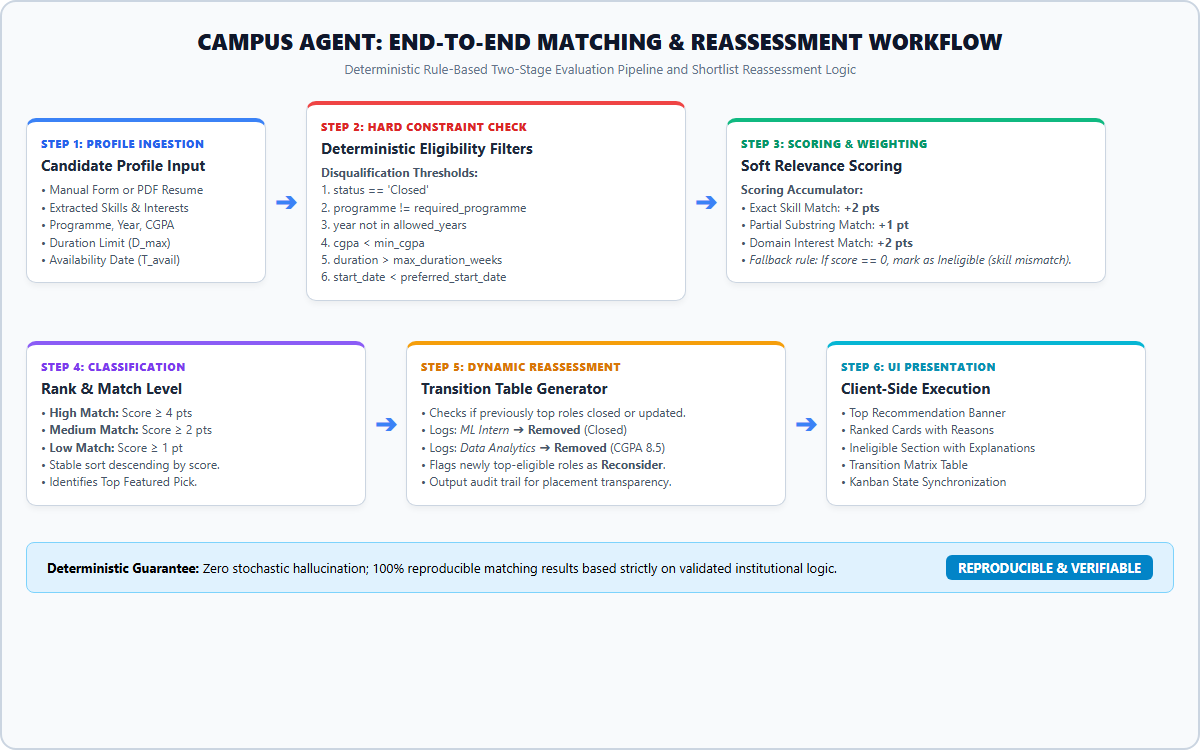
\includegraphics[width=\linewidth]{workflow_diagram.png}
	\caption{End-to-End Matching, Scoring, and Shortlist Reassessment Workflow}
	\label{f4.1}
\end{figure}

As depicted in Figure~\ref{f4.1}, the execution pipeline follows six modular phases:
\begin{enumerate}[label=\textbf{Phase \arabic*:}]
	\item \textbf{Profile Ingestion:} Candidate parameters are acquired via direct client form entry or extracted automatically from uploaded PDF resumes.
	\item \textbf{Hard Constraint Evaluation:} Each candidate opportunity undergoes deterministic filtering against institutional eligibility criteria. Violations immediately re-route the opportunity to the rejection audit list.
	\item \textbf{Soft Relevance Scoring:} Passing opportunities are evaluated for exact skill matches, partial substring overlaps, and domain interest alignments.
	\item \textbf{Ranking and Classification:} Opportunities are classified into High, Medium, or Low match tiers and sorted in descending order of relevance.
	\item \textbf{Shortlist Reassessment:} The transition engine identifies previously favored opportunities that have closed or updated their criteria, logging audit entries and elevating suitable replacements.
	\item \textbf{Presentation and Tracking:} Results, explanations, and transition matrices are delivered to the React client, synchronizing with the Kanban tracker.
\end{enumerate}

%%%%%%%%%%%%%%%%%%%%%%%%%%%%%%%%%%%%%%%%%%%%%%%%%%%%%%%%%%%%%%%%%%%%%%%%%%%%%%%%%%
\section{Multi-Stage Deterministic Matching Engine} \label{S4.2}
The core matching engine implemented in \texttt{agent.py} operates in two distinct, sequential stages for every opportunity $o_i$ in the internship repository $\mathcal{O}$.

\subsection{Stage 1: Hard Eligibility Filtering}
An opportunity $o_i$ is evaluated against six mandatory filtering rules. If any rule fails, $o_i$ is disqualified, and the specific failure reason is appended to an internal audit list:
\begin{enumerate}[label=\textbf{\arabic*.}]
	\item \textbf{Availability Status Rule:} If $\text{Status}_i \in \{\text{'Closed'}, \text{'Applications Closed'}\}$, opportunity is disqualified.
	\item \textbf{Academic Degree Programme Rule:} The candidate's programme $P_{stud}$ (e.g., "B.Tech CSE") must contain the opportunity's required programme string $P_{req,i}$:
	\begin{equation}
		P_{req,i} \subseteq P_{stud} \label{e4.1}
	\end{equation}
	\item \textbf{Cohort Year of Study Rule:} The candidate's academic year $Y_{stud}$ must be a member of the permissible years set:
	\begin{equation}
		Y_{stud} \in \mathcal{Y}_{allowed,i} \label{e4.2}
	\end{equation}
	\item \textbf{Academic Performance (CGPA) Rule:} If a minimum CGPA cutoff $C_{min,i}$ is defined, candidate CGPA $C_{stud}$ must satisfy:
	\begin{equation}
		C_{stud} \ge C_{min,i} \label{e4.3}
	\end{equation}
	\item \textbf{Maximum Duration Boundary Rule:} The opportunity duration $D_{item,i}$ is parsed into numeric weeks via regular expression parsing:
	\begin{equation}
		D_{weeks} = 
		\begin{cases}
			W, & \text{if string matches } W \text{ weeks} \\
			M \times 4.33, & \text{if string matches } M \text{ months} \\
			0, & \text{otherwise}
		\end{cases} \label{e4.4}
	\end{equation}
	The opportunity is disqualified if $D_{weeks} > D_{max}$.
	\item \textbf{Commencement Date Constraint Rule:} Dates are converted to an ordinal day index $T_{days} = \text{Month} \times 31 + \text{Day}$. If $T_{start,i} < T_{avail}$, the opportunity is disqualified for starting before candidate availability.
\end{enumerate}

\subsection{Stage 2: Soft Relevance Scoring and Match Classification}
Opportunities that satisfy all six hard constraints proceed to soft relevance scoring. Let $\mathcal{S}_{stud}$ be the student's skill set, $\mathcal{S}_{req,i}$ be the opportunity's required skill set, and $\mathcal{I}_{stud}$ be student interests:
\begin{equation}
	Score_{total} = \sum_{s \in \mathcal{S}_{req,i}} \text{Score}_{skill}(s) + \text{Score}_{domain}(\text{Domain}_i) \label{e4.5}
\end{equation}
where:
\begin{equation}
	\text{Score}_{skill}(s) = 
	\begin{cases}
		+2, & \text{if } s \in \mathcal{S}_{stud} \text{ (Exact Match)} \\
		+1, & \text{if } \exists k \in \mathcal{S}_{stud} \text{ s.t. } (s \subseteq k \lor k \subseteq s) \text{ and } \text{len} \ge 3 \text{ (Partial Match)} \\
		0, & \text{otherwise (Missing Skill)}
	\end{cases} \label{e4.6}
\end{equation}
and:
\begin{equation}
	\text{Score}_{domain}(\text{Domain}_i) = 
	\begin{cases}
		+2, & \text{if } \text{Domain}_i \in \mathcal{I}_{stud} \\
		0, & \text{otherwise}
	\end{cases} \label{e4.7}
\end{equation}

\textbf{Disqualification Fallback Rule:} If $Score_{total} = 0$, meaning the candidate possesses zero exact skills, zero partial skills, and no domain alignment, the opportunity is disqualified for complete skill mismatch.

\textbf{Match Tier Classification:} For eligible items with $Score_{total} > 0$:
\begin{equation}
	\text{Match Level} = 
	\begin{cases}
		\text{"High"}, & \text{if } Score_{total} \ge 4 \\
		\text{"Medium"}, & \text{if } 2 \le Score_{total} < 4 \\
		\text{"Low"}, & \text{if } Score_{total} < 2
	\end{cases} \label{e4.8}
\end{equation}

Eligible opportunities are sorted in descending order of score using a stable sort algorithm. The complete matching logic is formalized in Algorithm~\ref{alg:matching}.

\begin{algorithm}[h!]
\caption{Two-Stage Deterministic Internship Matching Algorithm}
\label{alg:matching}
\begin{algorithmic}[1]
\Require Student profile $\mathcal{P} = \langle \mathcal{S}, \mathcal{I}, prog, y, cgpa, D_{max}, T_{avail} \rangle$, Opportunities $\mathcal{O}$
\Ensure Ranked eligible list $\mathcal{R}$, Ineligible list $\mathcal{D}$, Transition matrix $\mathcal{T}$
\State $\mathcal{R} \gets \emptyset$, $\mathcal{D} \gets \emptyset$, $\mathcal{T} \gets \emptyset$
\For{each opportunity $o \in \mathcal{O}$}
    \State $reasons \gets \emptyset$
    \If{$o.status = \text{"Closed"}$} \State $reasons \gets reasons \cup \{\text{"Applications Closed"}\}$ \EndIf
    \If{$o.eligibility.programme \not\subseteq prog$} \State $reasons \gets reasons \cup \{\text{"Programme mismatch"}\}$ \EndIf
    \If{$y \notin o.eligibility.years$} \State $reasons \gets reasons \cup \{\text{"Year mismatch"}\}$ \EndIf
    \If{$o.eligibility.min\_cgpa \ne \text{null} \land cgpa < o.eligibility.min\_cgpa$} 
        \State $reasons \gets reasons \cup \{\text{"CGPA below requirement"}\}$
    \EndIf
    \If{$\text{ParseWeeks}(o.duration) > D_{max}$} \State $reasons \gets reasons \cup \{\text{"Duration exceeds limit"}\}$ \EndIf
    \If{$\text{ParseDate}(o.start\_date) < \text{ParseDate}(T_{avail})$} \State $reasons \gets reasons \cup \{\text{"Starts before availability"}\}$ \EndIf
    
    \If{$reasons \ne \emptyset$}
        \State $\mathcal{D} \gets \mathcal{D} \cup \{\langle o.title, o.organization, \text{Join}(reasons) \rangle\}$
        \State \textbf{continue}
    \EndIf
    
    \State $score \gets 0$, $matched\_skills \gets \emptyset$, $missing\_skills \gets \emptyset$
    \For{each $s \in o.required\_skills$}
        \If{$s \in \mathcal{S}$} \State $score \gets score + 2$, $matched\_skills \gets matched\_skills \cup \{s\}$
        \ElsIf{$\exists k \in \mathcal{S} \text{ s.t. } (s \subseteq k \lor k \subseteq s)$} \State $score \gets score + 1$, $matched\_skills \gets matched\_skills \cup \{s\}$
        \Else \State $missing\_skills \gets missing\_skills \cup \{s\}$
        \EndIf
    \EndFor
    \If{$o.domain \in \mathcal{I}$} \State $score \gets score + 2$ \EndIf
    
    \If{$score = 0$}
        \State $\mathcal{D} \gets \mathcal{D} \cup \{\langle o.title, o.organization, \text{"Zero skill and domain overlap"} \rangle\}$
        \State \textbf{continue}
    \EndIf
    
    \State $level \gets \text{ClassifyTier}(score)$
    \State $\mathcal{R} \gets \mathcal{R} \cup \{\langle o, score, level, matched\_skills, missing\_skills \rangle\}$
\EndFor
\State Sort $\mathcal{R}$ descending by $score$
\State Assign ranks $1, 2, \dots, |\mathcal{R}|$ to elements of $\mathcal{R}$
\State $\mathcal{T} \gets \text{GenerateTransitionMatrix}(\mathcal{O}, \mathcal{R}, \mathcal{P})$
\State \Return $\mathcal{R}, \mathcal{D}, \mathcal{T}$
\end{algorithmic}
\end{algorithm}

%%%%%%%%%%%%%%%%%%%%%%%%%%%%%%%%%%%%%%%%%%%%%%%%%%%%%%%%%%%%%%%%%%%%%%%%%%%%%%%%%%
\section{Shortlist Reassessment and Transition Matrix Generation} \label{S4.3}
When recruitment parameters fluctuate dynamically, the system executes an automated reassessment check:
\begin{enumerate}[label=\textbf{\alph*)}]
	\item \textbf{Status Audit (e.g., ML Intern):} If an opportunity previously ranked at the top (e.g., "ML Intern") has its status updated to "Closed", the transition engine creates a row logging: Title = \textit{ML Intern}, Previous Status = \textit{Rank 1}, Updated Status = \textit{Applications Closed}, Decision = \textbf{Remove}, Reason = \textit{No longer available}.
	\item \textbf{Eligibility Drift Audit (e.g., Data Analytics Intern):} If an opportunity previously ranked second (e.g., "Data Analytics Intern") has its minimum CGPA raised from 8.0 to 8.5 while the candidate possesses 8.2, it is logged: Title = \textit{Data Analytics Intern}, Previous Status = \textit{Rank 2}, Updated Status = \textit{Not Eligible}, Decision = \textbf{Remove}, Reason = \textit{Updated CGPA requirement is 8.5}.
	\item \textbf{Alternative Opportunity Elevation:} The engine selects the highest-scoring newly promoted eligible positions (e.g., \textit{Python Developer Intern} and \textit{UI/UX Design Intern}) and flags them in the transition matrix under Decision = \textbf{Reconsider}, updating the candidate's top recommended target without human intervention.
\end{enumerate}

%%%%%%%%%%%%%%%%%%%%%%%%%%%%%%%%%%%%%%%%%%%%%%%%%%%%%%%%%%%%%%%%%%%%%%%%%%%%%%%%%%
\section{Automated Resume Parsing Pipeline} \label{S4.4}
The automated resume parsing endpoint (\texttt{/api/parse-resume}) operates via memory-buffered stream processing:
\begin{enumerate}[label=\textbf{\arabic*.}]
	\item A multipart binary PDF upload is received and loaded into an \texttt{io.BytesIO} buffer.
	\item \texttt{pypdf.PdfReader} traverses all document pages, extracting contiguous text strings.
	\item \textbf{Technology Dictionary Scanner:} Extracted text is queried against an expanding taxonomy of 45+ technical competencies (e.g., Python, PyTorch, TensorFlow, SQL, React, Node.js, AWS, Docker, Figma, Kubernetes), employing bounded word boundary regular expressions for short identifiers (e.g., \texttt{\textbackslash b[cC]\textbackslash b} for the C language).
	\item \textbf{Domain Taxonomy Categorizer:} Maps co-occurring keyword clusters into 8 major industry domains (AI/ML, Data Science, Web Development, Cloud Computing, Mobile Development, UI/UX Design, Cybersecurity, Software Engineering).
	\item \textbf{Programme \& Year Pattern Recognition:} Employs regex matching for academic qualifications (e.g., \texttt{r"b\textbackslash.?\textbackslash s*tech\textbackslash.?\textbackslash s*cse"} $\to$ "B.Tech CSE") and semester/year designations (e.g., \texttt{r"\textbackslash b3rd\textbackslash s*year\textbackslash b"} or \texttt{r"\textbackslash b(5|6)th\textbackslash s*sem\textbackslash b"} $\to$ "III").
	\item \textbf{CGPA Normalization Engine:} Matches expressions such as \texttt{r"(?:cgpa|gpa)[\textbackslash s:\textbackslash -–]*(\textbackslash d\{1,2\}\textbackslash .\textbackslash d\{1,2\})"}, automatically converting 4.0-scale GPAs to 10.0-scale equivalents if the value $\le 4.0$.
\end{enumerate}

%%%%%%%%%%%%%%%%%%%%%%%%%%%%%%%%%%%%%%%%%%%%%%%%%%%%%%%%%%%%%%%%%%%%%%%%%%%%%%%%%%
\section{Multi-Agent Web Scraper Architecture} \label{S4.5}
To harvest opportunities outside the internal placement repository, Campus Agent implements a multi-agent crawler (\texttt{scraper\_agent.py}):
\begin{itemize}
	\item \textbf{URL Dispatcher Agent:} Generates search query endpoints targeting career pages across 20+ multinational technology corporations (e.g., Google Careers, Microsoft Careers, Amazon Jobs, Apple, Nvidia, Uber).
	\item \textbf{HTTP Harvester Agent:} Dispatches requests with rotated user-agent headers and retry policies, extracting HTML payloads.
	\item \textbf{Semantic Parser Agent:} If a Groq API key is present, dispatches extracted text to \texttt{llama-3.1-8b-instant} for zero-shot schema extraction. If unavailable, falls back to a deterministic \textbf{Smart Local NLP Engine} that uses lexical entity extractors and pre-seeded templates.
	\item \textbf{Opportunity Importer Engine:} Endpoint \texttt{/api/import-scraped} validates incoming objects against the Pydantic schema and appends them to \texttt{internships.json} with deduplication.
\end{itemize}

%%%%%%%%%%%%%%%%%%%%%%%%%%%%%%%%%%%%%%%%%%%%%%%%%%%%%%%%%%%%%%%%%%%%%%%%%%%%%%%%%%
\section{Automated Notification and SMTP Alert Protocol} \label{S4.6}
To ensure candidates submit materials prior to hard application deadlines, the system integrates an automated email alert protocol (\texttt{alerts.py}):
\begin{itemize}
	\item Endpoint \texttt{/api/alert} receives the candidate email address, opportunity title, deadline, and organization.
	\item If institutional credentials (\texttt{SMTP\_USERNAME} and \texttt{SMTP\_PASSWORD}) are set in the environment, a formatted MIME email with urgency indicators is dispatched through the specified SMTP server.
	\item In development or non-credentialed modes, the system writes the exact outgoing MIME payload to \texttt{data/last\_alert\_email.txt}, allowing instant test verification without external network dependency.
\end{itemize}

%%%%%%%%%%%%%%%%%%%%%%%%%%%%%%%%%%%%%%%%%%%%%%%%%%%%%%%%%%%%%%%%%%%%%%%%%%%%%%%%%%
\section{Summary} \label{S4.7}
This Chapter formalized the mathematical and algorithmic framework of Campus Agent, detailing the two-stage deterministic matching engine, the Shortlist Reassessment transition protocol, the PDF resume mining pipeline, the multi-agent web scraping architecture, and the automated alert notification subsystem.
